\section{Data Mining}
\label{dm}
Die vorliegende wissenschaftliche Fragestellung bewegt sich im Bereich des Data Minings. Das folgende Kapitel soll dem Leser dazu eine Einführung in die Thematik geben, um ein Verständnis der grundlegenden Begrifflichkeiten und Ziele des Data Minings zu erhalten (vgl. \vref{defdm}). Darüber hinaus werden die Prozesse des Data Minings (vgl. \vref{prozdm}) beleuchtet, wobei der \textit{Knowledge Discovery in Data} Prozess -- methodischer Aufbau der späteren Umsetzung -- in \vref{kdd} nochmal ausführlich erläutert wird.

\subsection{Definition des Data Minings}
\label{defdm}

Der Begriff des Data Minings reicht zurück bis in die 80er-Jahre des letzten Jahrhunderts und verfolgt das Ziel, Wissen aus umfassenden Datenmengen zu extrahieren.\seFootcite{Vgl.}{S. 2}{Runkler.2015} Es handelt sich um einen Prozess des \glqq  \textit{Sammelns, Säuberns, Verarbeitens und Analysierens von Daten, zur Gewinnung von nützlichen Informationen.}\grqq\seFootcite{}{S. 1}{Aggarwal.2015} Der weltweit gesammelte Datenbestand erhöht sich immer mehr und stellt Analysten vor die Herausforderung, aus dieser Datenflut wertvolle Informationen und organisiertes Wissen abzuleiten.

Erst das heutige \glqq Informationszeitalter\grqq~führte zum Beginn des renommierten Wissenschaftsbereiches des Data Minings, welcher in der Literatur auch als \glqq natürliche Evolution\grqq~der Informationstechnologie bezeichnet wird.\seFootcite{Vgl.}{S. 1}{Garcia.2015}\seFootcite{Vgl.}{S. 2}{Han.2012} Grundlegende interdisziplinäre, wissenschaftliche Teilgebiete des Data Minings sind z.B. die Statistik, das maschinelle Lernen (\gls{ml}), die Mustererkennung, die Systemtheorie sowie die \gls{ki}.\seFootcite{Vgl.}{S. 2}{Runkler.2015}\seFootcite{Vgl.}{S. 1}{Shi.2015}


Cleve und Han vergleichen die Suche nach Mustern und Zusammenhängen in den Daten mit dem Abbau von Rohstoffen.\footnote{Die englische Übersetzung lautet \textit{\glqq Mining\grqq}} Sowie im Bergbau nach Schätzen wie Gold und Silber im Gestein gesucht wird, so strebt das \gls{dm} nach dem Ableiten von Wissen aus (Roh-)Daten.\seFootcite{Vgl.}{S. 1}{Cleve.2014}\seFootcite{Vgl.}{S. 5-6}{Han.2012} Han geht sogar einen Schritt weiter und präferiert den Begriff des \textit{Knowledge Minings from Data} -- bezogen auf den verwendeten Terminus des \textit{Gold Minings}, statt den des \textit{Rock or Sand Minings} -- da diese Bezeichnung das eigentliche Ziel, die Gewinnung von Wissen, beinhaltet.\seFootcite{Vgl.}{S. 5-6}{Han.2012}\footnote{Weitere Termini nach Han: \textit{knowledge mining from data, knowledge extraction, data/pattern analysis, data archaeology, and data dredging.}}

\glqq Unter Wissen verstehen wir interessante Muster, die allgemein gültig sind, nicht trivial, [sondern] neu, nützlich und verständlich.\grqq\seFootcite{}{S. 2}{Runkler.2015} Insofern wird das Ziel verfolgt, komplexe Paradigmen zu erkennen, die durch bloße Betrachtung der Daten nicht aufgedeckt werden können. Oftmals fehlt dem Datenanalysten das spezifische Fachwissen zur Erkennung von Mustern, sodass durch die Einbeziehung von Experten ein iterativer Prozess entsteht, bis ein vorher definiertes Ziel erreicht wird. Zunächst werden aus den Daten Informationen gewonnen, aus welchen wiederum Wissen abgeleitet werden kann, wobei in diesem Prozess der Wissensextraktion die Datenmenge sukzessive abnimmt und sich verdichtet, wie \vref{wissenprozess} verdeutlicht.

\begin{figure}[H]
\centering
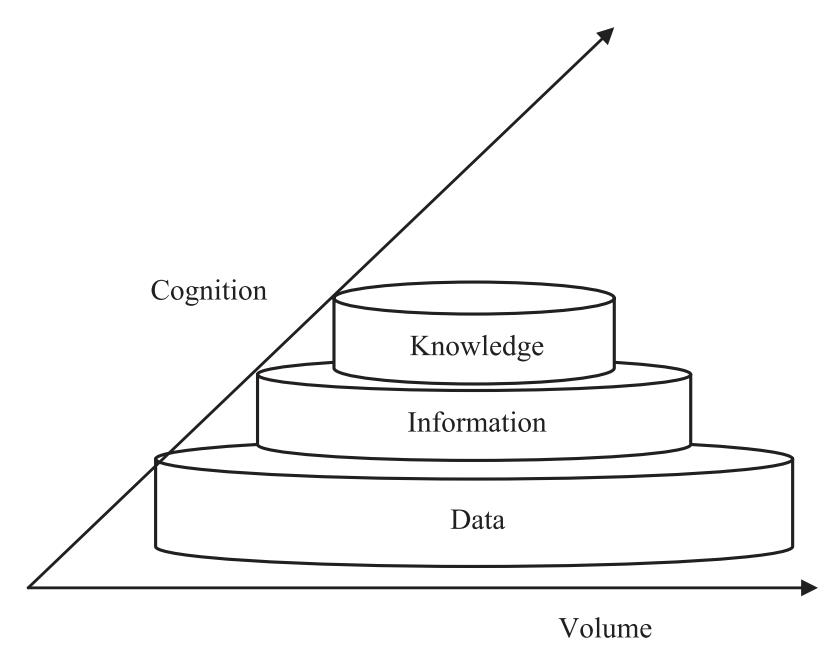
\includegraphics[scale=1.3]{se-wa-jpg/wissenprozess}
\caption[Wissensextraktion aus Daten]{Wissensextraktion aus Daten\protect\footnotemark}
\label{wissenprozess}
\end{figure}
\footnotetext{Vgl. Abbildung \textit{Shi} et al., Intelligent Knowledge, 2015, S. 5.}

\textit{Daten} stellen dabei nur eine Reihe von Zeichen dar, wobei deren Bedeutung zunächst unklar ist. Erst wenn bekannt wird, in welchem Kontext die Daten stehen und welche Beziehungen zwischen diesen besteht, können diese interpretiert werden und zu einer (relevanten) \textit{Information} heranwachsen. Das \textit{Wissen} entsteht letztlich durch die Verknüpfung von den vielen Daten und Informationen, sowie den damit gesammelten Erfahrungen.\seFootcite{Vgl.}{S. 16-18}{Shi.2015}

Durch den Einsatz von modernster Computerhard- als auch Software ist es möglich, sehr große Datenmengen zu erheben, zu verarbeiten und zu analysieren, wodurch in diesem Kontext der Begriff \gls{bigdata} entstanden ist.\seFootcite{Vgl.}{S. 3}{Witten.2011} \gls{bigdata} bezeichnet Datenmengen, die mit herkömmlichen Analysemethoden nicht mehr zu verarbeiten sind und deshalb die Anwendung des Data Minings benötigen.\seFootcite{Vgl.}{S. 5}{Fasel.2016}\seFootcite{Vgl.}{S. 1}{Shi.2015} Hierzu einige ausgewählte Beispiele aus verschiedenen Datenbereichsquellen:\seFootcite{Vgl.}{S. 2}{Aggarwal.2015}

\begin{itemize}
\item \textbf{World Wide Web:} Die Anzahl der Dokumente im Internet hat seit langem die Milliarden-Marke geknackt, wobei die des unsichtbaren \glqq Webs\grqq~noch viel größer ist. Durch Nutzerzugriffe auf Inhalte, werden auf Serverseite Log-Dateien kreiert, um beispielsweise die Auslastung und Zugangszeiten zu protokollieren. Andererseits wird das Kundenverhalten auf kommerziellen Seiten aufgezeichnet, um personalisierte Werbung schalten zu können.

\item \textbf{Benutzerinteraktion:} Festnetzanbieter nutzen die durch Telefonate entstandenen Daten wie Gesprächslänge und -ort, um relevante Muster über die Netzwerksauslastung, zielgerichtete Werbung oder auch anzusetzende Preise durch Datenanalyse zu extrahieren.
\item \textbf{Internet of Things:} Durch kostengünstige (tragbare) Sensoren und deren kommunikative Vernetzung, entstand das \gls{iot}. Einer der Trends der heutigen Informationstechnologie, welcher durch die Erhebung von Massendaten eine signifikante Rolle für das Data Mining einnimmt.

\item \textbf{Weitere Beispiele:}  Social Media Plattformen (allen voran Facebook, Twitter und Co.), Finanzmärkte (z.B. der Aktienmarkt), Sport (z.B. Baseball, Basketball, Football oder wie in dieser Arbeit Fußball), uvm.\seFootcite{Vgl.}{S. 39}{Fayyad.1996}\seFootcite{Vgl.}{S. 1-2}{Han.2012}\seFootcite{Vgl.}{S. 85 ff}{Chu.2014} 
\end{itemize}

\glqq Wir befinden uns in einer Welt, in der wir reich an Daten sind, jedoch arm an Informationen und Wissen.\grqq\seFootcite{}{S. 5}{Han.2012} Der unglaublich rapide und enorme Datenzuwachs hat bei Weitem unsere menschliche Vorstellungskraft und Möglichkeiten übertroffen, sodass wir auf effiziente Werkzeuge angewiesen sind (siehe \vref{dmmethoden}). Die sich immer weiter ausbreitende Lücke zwischen Daten und Informationen, führt nur noch durch die Anwendung von Methoden des Data Minings zu den begehrten \glqq \textit{Golden Nuggets of Knowledge}\grqq.\seFootcite{Vgl.}{S. 5}{Han.2012} Dazu müssen die (Roh-)Daten gezielt ausgewählt und umstrukturiert werden, um diese anschließend durch Algorithmen analysieren zu können. Folglich entstanden Data Mining Prozesse, die dieses Problem mit Hilfe systematischer Abläufe lösen sollen (vgl. \vref{prozdm}). Zudem wird \glqq Data Mining [...] heute durch eine zunehmende Anzahl von Software-Tools unterstützt. Dazu zählen unter anderem Software-Lösungen wie: KNIME, MATLAB, SPSS, SAS, STATISTICA, TIBCO Spotfire, R, Rapid Miner, Tableau, QlikView, oder WEKA.\grqq\seFootcite{Vgl.}{S. 3}{Runkler.2015} Das Software-Tool \textit{MatLab} wird innerhalb der Funktionsmodellierung in \vref{fm} vorgestellt und anschließend als Werkzeug zur Anwendung von Data Mining Methoden in der Umsetzungsphase genutzt (vgl. \vref{umsetzung}).


\subsection{Data Mining Prozesse}
\label{prozdm}

In der Literatur grenzen viele Wissenschaftler den Begriff des eigentlichen Data Minings, vom Gesamtprozess der Extraktion von Wissen ab. Andere wiederum behandeln beide Termini synonym zueinander.\seFootcite{Vgl.}{S. 39}{Fayyad.1996}\seFootcite{Vgl.}{S. 2}{Mariscal.2010}\seFootcite{Vgl.}{S. 1}{Garcia.2015} Schlechte Qualität der Daten mindert die Leistungsfähigkeit des Data Minings. Um die Aussagekraft der Daten nicht zu gefährden, sind vorab Prozessschritte notwendig, die die Daten in adaptierter Form für die Methoden des Data Minings bereitstellen.\seFootcite{Vgl.}{S. 10}{Garcia.2015} Hierzu werden im Folgenden kurz die zwei bekanntesten Prozessmodelle vorgestellt:

\begin{itemize}
\item \gls{kdd}
\item \gls{crisp-dm}
\end{itemize}

\subsubsection{Knowledge Discovery in Data}
\label{dmkdd}

Der Begriff des \textit{Knowledge-Discovery-in-Data}-Prozesses wurde in den frühen 90er-Jahren geprägt und wird als \glqq nicht trivialer Prozess zur Identifizierung von gültigen, neuartigen, potentiell sinnvollen und letztlich verständlichen Mustern in Daten\grqq\seFootcite{}{S. 41}{Fayyad.1996} definiert.\seFootcite{Vgl.}{S. 2}{Mariscal.2010} Erstmals wurde der Terminus von Gregory Piatetsky-Shapiro auf der \textit{International Joint Conference on Artificial Intelligence}, 1989 in Detroit (USA), der Öffentlichkeit präsentiert.\seFootcite{Vgl.}{S. 1}{Adhikari.2015} Der in \vref{kddpic} dargestellte iterative \gls{kdd}-Prozess nach Fayyad, beinhaltet folgende Schritte, wobei das \gls{dm} als ein eigener Prozessschritt ausgewiesen wird:\seFootcite{Vgl.}{S. 5}{Cleve.2014}

\begin{enumerate}

\item \textbf{Datenselektion}: Auswahl der geeigneten Datenmengen.
\item \textbf{Datenvorverarbeitung}: Behandlung fehlender oder problembehafteter Daten.
\item \textbf{Datentransformation}: Umwandlung in adäquate Datenformate.
\item \textbf{Data Mining}: Suche nach Mustern.
\item \textbf{Interpretation und Evaluation}: Interpretation der Ergebnisse und Auswertung dieser.

\end{enumerate}

Auf die einzelnen Prozessschritte und deren Methoden wird genauer in \vref{kdd} eingegangen. Die Abkürzung \textit{KDD} steht in der Literatur für unterschiedliche Bezeichnungen, wie zum Beispiel \textit{Knowledge Discovery in Databases}, \textit{Knowledge Discovery in Data Mining} oder \textit{Knowledge Discovery in Data Warehouses}.\seFootcite{Vgl.}{S. 26 ff}{OseiBryson.2015} Alle zielen dabei auf die Erforschung von Wissen aus Datenmengen ab, wofür in dieser Arbeit die allgemeingültige Bezeichnung \textit{Knowledge Discovery in Data} verwendet wird.

\begin{figure}[H]
\centering
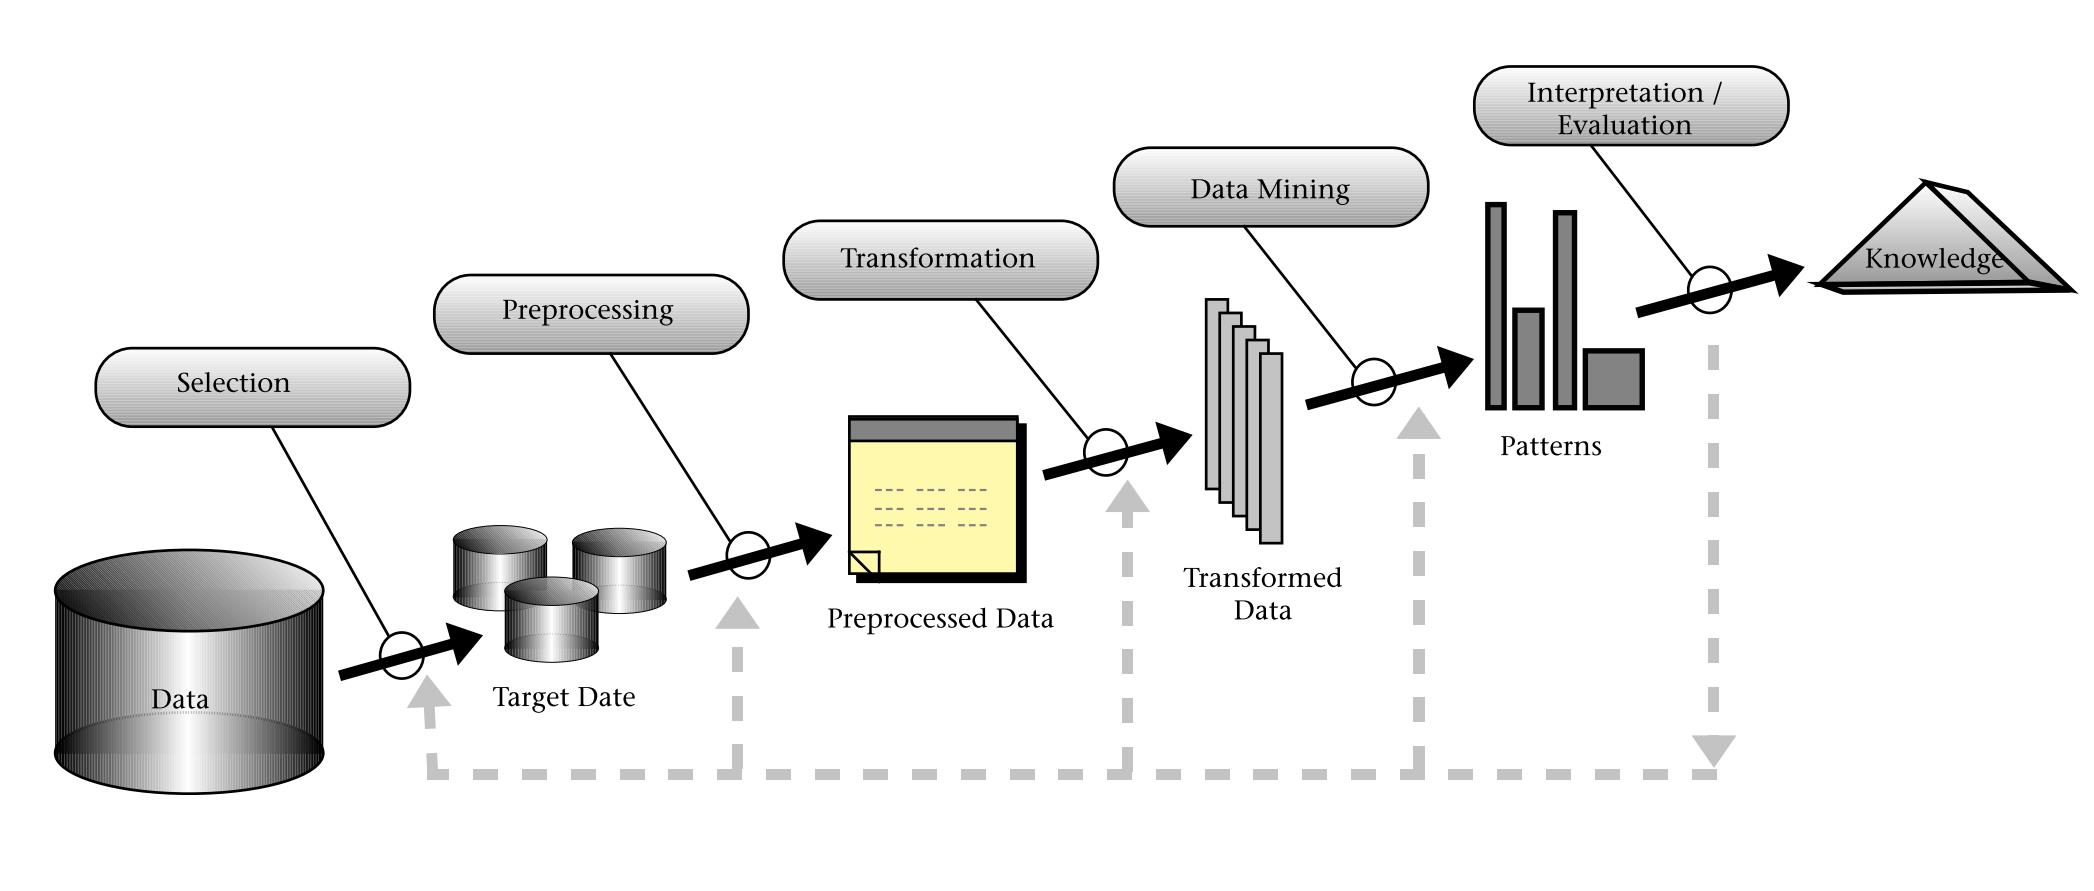
\includegraphics[scale=0.85]{se-wa-jpg/kdd}
\caption[Der Knowledge Discovery in Data Prozess]{Der Knowledge Discovery in Data Prozess\protect\footnotemark}
\label{kddpic}
\end{figure}
\footnotetext{Vgl. Abbildung \textit{Fayyad} et al., From Data Mining to Knowledge, 1996, S. 41.}


\subsubsection{CRISP-DM}
Das \gls{crisp-dm}-Modell wurde im Jahr 2000 durch ein Konsortium, bestehend aus mehreren nachfolgenden aufgeführten Firmen, entwickelt.\seFootcite{Vgl.}{S. 6}{Cleve.2014}\seFootcite{Vgl.}{S. 3}{Mariscal.2010}

\begin{itemize}
\item NRC Corporation
\item Daimler AG
\item SPSS Inc.
\item Teradata 
\item OHRA
\end{itemize}

Dieses Modell verfolgt das Ziel, einen standardisierten und branchenübergreifenden Data-Mining-Prozess zu definieren und das dadurch berechnete Modell zu validieren. Hierbei wird von einem Lebenszyklus, bestehend aus sechs Etappen, ausgegangen, der in \vref{crisp} dargestellt wird.\seFootcite{Vgl.}{S. 6-8}{Cleve.2014} Im Folgenden werden dazu die einzelnen Schritte des Prozesses aus der Abbildung (nummeriert von Schritt 1 bis 6) kurz erläutert.

\begin{figure}[H]
\centering
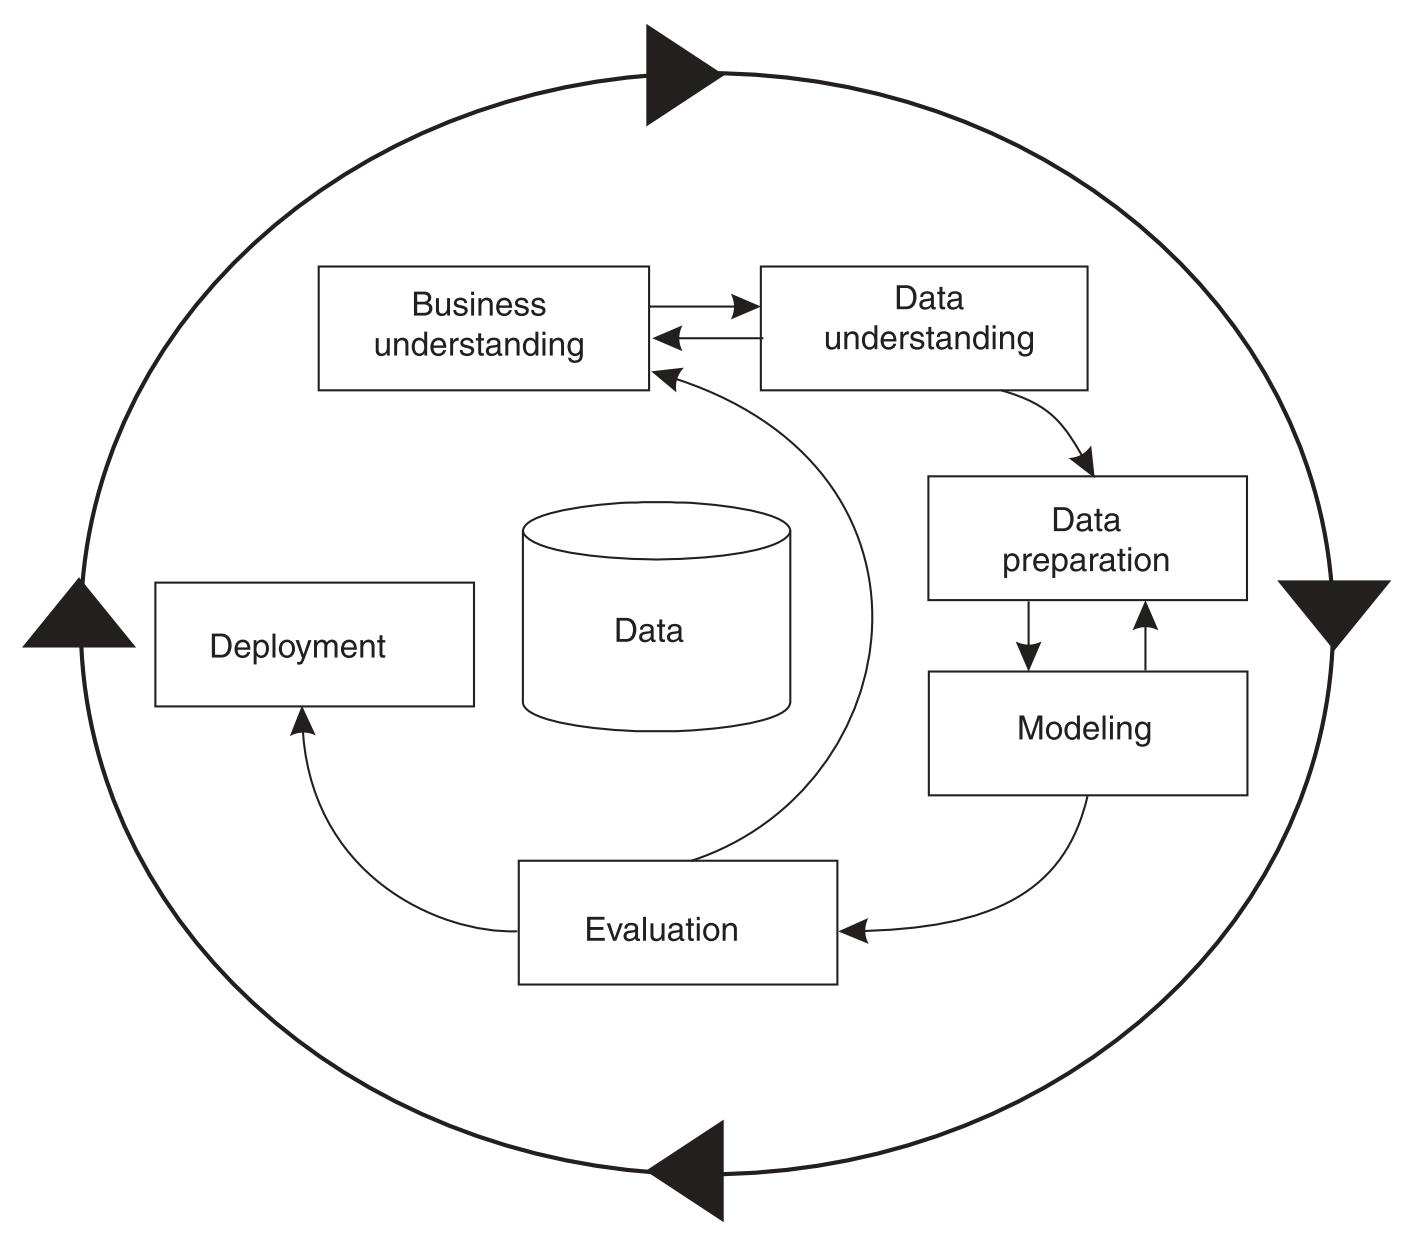
\includegraphics[scale=0.9]{se-wa-jpg/crisp}
\caption[CRISP-DM Prozess]{CRISP-DM Prozess\protect\footnotemark}
\label{crisp}
\end{figure}
\footnotetext{Vgl. Abbildung \textit{Mariscal} et al., A survey of data mining, 2010, S. 13}

\paragraph{1. Verstehen der Aufgabe}(\textit{Business understanding}): 
Hier steht das grundsätzliche Verständnis des Fachgebietes und der Aufgabe im Vordergrund. Die Ziele werden definiert, Ressourcen des Unternehmens ermittelt und die Ausgangssituation bestimmt. Weiterhin müssen Erfolgskriterien quantifiziert und Risiken eruiert werden, um eine Kostenplanung aufstellen zu können. 
\paragraph{2. Verständnis der Daten}(\textit{Data understanding}): 
Diese Phase beschäftigt sich mit den benötigten Daten zur Durchführung der Analyse. Daten werden gesammelt und beschrieben, um deren betrieblichen Kontext, indem sie stehen, zu verstehen.
\paragraph{3. Datenvorbereitung}(\textit{Data preparation}): 
Es gilt den Data-Mining-Prozess-Schritt vorzubereiten, wobei fehlerhafte und inkonsistente Daten korrigiert werden müssen, um diese schließlich in eine Datenstruktur transformieren zu können, die für die Methoden des Data Minings nutzbar sind.
\paragraph{4. Data Mining - Modellbildung}(\textit{Modeling}): 
In dieser Phase wird ein Modell mit Hilfe des Data Minings erstellt, welches durch einen iterativen Aufbau immer wieder verfeinert und verbessert wird. 
\paragraph{5. Evaluation:}
Die erzielten Ergebnisse werden an den aus Phase 1 definierten Erfolgskriterien gemessen, um festzustellen, ob der wirtschaftliche Nutzen erzielt wird.
\paragraph{6. Einsatz im Unternehmen}(\textit{Deployment}): 
Zuletzt gilt es, den Einsatz der Resultate im Unternehmen vorzubereiten und diese in das operative Geschäft zu integrieren.

Das Modell bezieht und orientiert sich, wie schon am Namen zu erkennen ist, stark an wirtschaftlichen Projekten und beschreibt \textit{Was} zu tun ist, jedoch nicht genau \textit{Wie}, sodass Projektteams innerhalb dieses Rahmens beginnen ihre eigenen Methoden zu entwickeln.\seFootcite{Vgl.}{S. 4}{Mariscal.2010}

Im Vergleich zum \gls{kdd}-Modell nach Fayyad, sind die Phasen 1 und 2 des \gls{crisp-dm}-Modells sehr stark projektabhängig und spiegeln die Sicht der Industrie auf das Projekt wider.\seFootcite{Vgl.}{S. 8}{Cleve.2014} Im Gegensatz dazu konzentriert sich der \gls{kdd}-Prozess auf die Datenbereitstellung und Analyse, sodass dieser als grundlegende Methodik für die spätere Umsetzung der wissenschaftlichen Aufgabenstellung herangezogen wird und genauer in \vref{kdd} beleuchtet wird.

Mariscal et al. diskutieren in ihrer Studie zahlreiche weitere Prozessmodelle zur Extraktion von Wissen aus riesigen Datenmengen, wobei die Kernelemente der Datenselektion, -vorverarbeitung und -tranformation, sowie der anschließende Schritt des eigentlichen Data Minings immer wieder aufzufinden sind.\seFootcite{Vgl. vorgestellte Modelle aus}{}{Mariscal.2010} Nicht zuletzt ist zu erwähnen, dass in der Literatur unterschiedliche Auffassungen zu dem Begriff des Data Minings existieren und dieser oftmals mit den Data Mining Prozessen synonym verwendet wird. Ein Hinweis darauf sind auch die weit über 500 wissenschaftlichen Artikel zu dem Journal \textit{Data Mining and Knowledge Discovery} auf \textit{Springer Link}.

